%-*-latex-*-
\sectionthree{Algorithmic analysis: how fast is an algorithm?}
\begin{python0}
from solutions import *; clear()
\end{python0}

Why do we study asymptotics? For the computer scientists,
asymptotics tell us what to focus on and what to ignore.
It creates a useful classification of functions that grow in the
same manner. 

For instance look at the following algorithm that
computes the sum of integers from 1 to $n$ (the value of $n$ is
stored in variable $n$) and the sum is stored in
$s$.
\begin{Verbatim}[frame=single, fontsize=\footnotesize]
s = 0
for i = 1, 2, ..., n:
     s = s + i
\end{Verbatim}
This algorithm solves the following problem:
\[
P(n): \text{\lq\lq Compute the sum of integers from $1$ to $n$''}
\]
This problem is of course made up of many specific problem instances.
For example it includes: 
\[
P(10): \text{\lq\lq Compute the sum of integers from $1$ to $10$''}
\]
and
\[ 
P(1135452): \text{\lq\lq Compute the sum of integers from $1$ to $1135452$''}
\]

Our algorithm:
\begin{Verbatim}[frame=single, fontsize=\footnotesize]
s = 0
for i = 1, 2, ..., n:
     s = s + i
\end{Verbatim}
is an algorithmic solution to our problem $P(n)$.
(It's not the only one.)

In the above, you can think of $n$ as the \textit{size} of each problem
instance.
And of course you would expect, without even analyzing our
algorithm in detail, that the above algorithm will need more time
for a large $n$. Correct?

Different people design different algorithms to solve the same problem.

We are interested in measuring how fast an algorithm runs
so that we can pick the best.
It's clear that the crucial thing to focus on is the performance
of an algorithm when $n$ is large.
After all, the sum from 1 to 3 is easy --
in fact we can do $1+2+3$ in our heads and not bother with
running a program at all, right?
It takes more time just to let your computer boot up or wake up!!!

In the real world, 
after the algorithm is designed (and you've checked that it's 
correct!!!), 
you still have to implement the algorithm with a programming language
and run the program on a specific computer.
In the real world, the performance of the algorithm can be measured by the
time taken by the computer to run the program.
By \lq\lq time taken'' in this case, I mean measuring time with a
watch or the clock.
This is sometimes called \defone{wall-clock time}.

On some OS, you can also measure processor time for a program, i.e.,
the amount of time that the program actually uses the CPU.

However using the wall-clock or processor time
is problematic because
it depends on the hardware used,
the programming language used,
the operating system, etc.
(No, it does not depend on how many planets are lined up.)

What I want to do is to measure the performance independent of 
external factors, i.e., I want to measure the performance of the 
algorithm.
This does not mean that the external factors are not important.
But rather, we want to solve the performance issue at the root first.
In fact this is usually \textit{the} most important factor in the 
performance of any software.

Now let's get back to our 
sum from 1 to $n$ algorithm and see how we can measure the 
runtime performance of an algorithm without even running it on a piece of
hardware.

I'm going to rewrite my algorithm like this (apologies
to those who disapprove of goto statements):
\begin{samepage}
\begin{Verbatim}[frame=single,fontsize=\footnotesize]
         s = 0                     
         i = 1                     
LOOP:    if i > n:                  
             goto ENDLOOP          
         s = s + i                 
         i = i + 1                 
         goto LOOP                 
ENDLOOP:
\end{Verbatim}
\end{samepage}
In this simplified language, we have basic operations
such as assignment operators, arithmetic operators (such as \verb!+!),
and boolean operators (such as \verb!>!).
Besides that we have goto statements and
conditional branching statements
\verb!if [boolean]: goto [label]!.
In the above pseudocode, I've implemented a for-loop using
a conditional branching and goto statement.
Control structures such as for-loops, while-loops, do-while loops,
if statements, 
and if-else statements are actually implemented at the machine code level
with goto and conditional branching statements (see CISS360).
Therefore goto and conditional branching statements are actually
more fundamental.

Now I'm going to attach time taken to execute each statements:
\begin{Verbatim}[frame=single,fontsize=\footnotesize]
                             time
         s = 0               t1 
         i = 1               t2 
LOOP:    if i > n:           t3  
             goto ENDLOOP    t4
         s = s + i           t5
         i = i + 1           t6
         goto LOOP           t7
ENDLOOP:
\end{Verbatim}
This is how you read the above time \lq\lq accounting'':
The statement 
\begin{Verbatim}[frame=single,fontsize=\footnotesize]
         s = 0               t1
\end{Verbatim}
takes $t_1$ seconds (or whatever unit of time
you like ... you'll see later that the specific value of 
$t_1$ and the units are not important at all).
For the \verb!if!--statement
(which is made of a header and a body):
\begin{Verbatim}[frame=single,fontsize=\footnotesize]
LOOP:    if i > n:           t3  
             goto ENDLOOP    t4
\end{Verbatim}
it takes time $t_3$ for the \verb!if!--statement
to compute the boolean value of $i > n$ and then to decide
to execute \verb!goto ENDLOOP! or not.
So if the boolean condition is true, then the time taken for the 
whole \verb!if! statement is $t_3 + t_4$;
if the boolean condition is false, then the time taken 
is $t_3$.

Note that the times taken to execute each of the above
statement, $t_1$, $t_2$, ... are
\textit{constants with respect to} $n$.
What this mumbo-jumbo meant was, 
whether I run the above algorithm
with $n = 10$ or $n = 1000000$, 
the time taken is this:
\begin{Verbatim}[frame=single,fontsize=\footnotesize]
         s = 0               t1
\end{Verbatim}
is still $t_1$.
Makes sense, right?

Next, we count the number of times each statement is executed:
\begin{Verbatim}[frame=single,fontsize=\footnotesize]
                             time    number of times
         s = 0               t1      1
         i = 1               t2      1
LOOP:    if i > n:           t3      n + 1
             goto ENDLOOP    t4      1
         s = s + i           t5      n     
         i = i + 1           t6      n     
         goto LOOP           t7      n
ENDLOOP:
\end{Verbatim}
For instance
\begin{Verbatim}[frame=single,fontsize=\footnotesize]
         s = 0               t1      1
\end{Verbatim}
is executed once (regardless of the value of $n$).
For the \verb!if!--statement
\begin{Verbatim}[frame=single,fontsize=\footnotesize]
LOOP:    if i > n:           t3      n + 1
             goto ENDLOOP    t4      1
\end{Verbatim}
since $i$ runs through 
$1$, $2$, ..., $n - 1$, $n$, $n + 1$
(the boolean condition evaluates to true for the first $n$
values and false for the last value of $n + 1$),
the header of the \verb!if! is executed $n + 1$ times
and the body is executed only once.

Finally (phew!) we compute the time taken to execute the code.
The total time taken is
\begin{align*}
  \text{Total time}
  &= t_1
  + t_2 
  + (n + 1) t_3 
  + t_4
  + n (t_5 + t_6 + t_7)
  \\
  &= (t_3 + t_5 + t_6 + t_7) n
  + (t_1 + t_2 + t_3 + t_4)  
\end{align*}
Therefore the total time taken is 
\[
An + B
\] 
for some constants
$A$ and $B$. 
Note that
$t_1,t_3,t_3, ...$, and therefore $A$ and $B$,
depends mainly on the machine that is executing the algorithm.

It's common to use $T(n)$ to denote the runtime of an algorithm.
So I might write:
\begin{align*}
  T(n)
  &=
  ( t_3 + t_5 + t_6 + t_7 )n
  + (t_1 + t_3 + t_3 + t_4)
  \\
  &= An + B
\end{align*}

If I'm talking about several algorithmic runtimes together
I would decorate the $T(n)$ notation.
For instance I might write
\[
T^P(n)
\]
or
\[
T^{\operatorname{sum-to}}(n)
\]
or
\[
T^{\operatorname{CONVERT-DIRT-TO-GOLD}}(n)
\]

Now as $n$ grows (and this is the situation we do want 
to worry about), $An$ is of course
going to be larger than $B$. 
So ultimately when $n$ is large the time taken to carry
out the algorithm is mainly and roughly due to $An$.
And since we don't really care to specify the hardware we're using,
we can also fudge away the constant $A$ and conclude the 
time take to run our algorithm or program is roughly 
(or rather proportional to) the function
\[
n
\]


The technical thing to do is this:
We write 
\[
T(n) = An+B = O(n)
\]
and say \lq\lq $T(n)$ is the big-O of $n$''.
The big-O tells the reader that 
we're only expressing what the runtime function looks like
for large $n$ and when we ignore multiples.
In this case I will say that this algorithm has
\defone{linear runtime}.
Instead of say \lq\lq the big-O runtime of the algorithm is $O(n)$",
you can also say the
\defone{time complexity} of the algorithm is $O(n)$.

\textsc{Warning:}
Make sure you see the difference between
\[
T(n) = O(n)
\]
and 
\[
T(n) = n 
\]
(which is wrong).

There are therefore \textit{two} elements to measuring the runtime
performance of an algorithm:
\begin{itemize}
\item[(1)] You need to be able to compute the runtime as a formula
in the size of the problem (which in the above is $n$)
\item[(2)] You need to do some fudging to get an \lq\lq approximation'',
  i.e., the big-O of the function from (1).
  If the formula from (1) is a sum of functions,
  you choose the one that is largest when $n$ is huge
  and you replace constants with $1$.
\end{itemize}

Notice in the above example, the fudging \textit{simplifies} the function from
\[
An + B
\]
to 
\[
n
\]

Now, as I said before,
I'm ignoring multiples so that 
I'm considering $An$ the same as $n = 1 \cdot n$.
Of course I could have chosen $2n$ as well.
But since I consider all multiples the same, I prefer to use $n$
since it's simpler than $2n$.

Let me summarize the above steps carried out in the computation
of the big-O of the runtime of our sum to $n$ algorithm:

STEP 1. First I assign times to each statement and 
compute the time taken to be
\begin{align*}
T(n)
 &= t_1 
    + t_2
    + (n + 1) t_3 
    + t_4
    + n (t_5 + t_6 + t_7)\\
 &= t_1
    + t_2 
    + t_3 
    + t_4 +
    n( t_3 + t_5 + t_6 + t_7 )
\end{align*}

STEP 2. I clean up and say 
that the time taken is a function of the form
\[
T(n) = An + B
\] 
where $A$ and $B$ are constants.

STEP 3.
The first fudging step is where I looked at the functions $An$ and $B$
and conclude that for large $n$, the function is roughly the function
\[
An
\]

STEP 4.
The second fudging step is when I throw away the $A$ (i.e., replace
the $A$ with $1$) because
the constant $A$ is hardware dependent and say that the 
time taken is roughly the function
\[
n
\]
and I conclude with this statement:
\[
T(n) = O(n)
\]

In general, to compute the big-O of any given function $f(n)$,
\begin{itemize}
\li You only keep the term that is the largest in the long run 
(i.e. for large $n$).
The growth of $f(n)$ is determined by this term.
Typically, your runtime function might have more than 2 terms.
\li You replace constant(s) by 1 because different constants
indicates different hardware being used.
\end{itemize}
Later we'll see that there are other simplifications and computational
tools.
The above steps are good enough for now.

OK, let me show you \textit{graphically} what the fudging does to a function.
Here are the plots of $y = 10n, y = 10n + 10, y = 10n + 50$:
%-*-latex-*-

\begin{center}
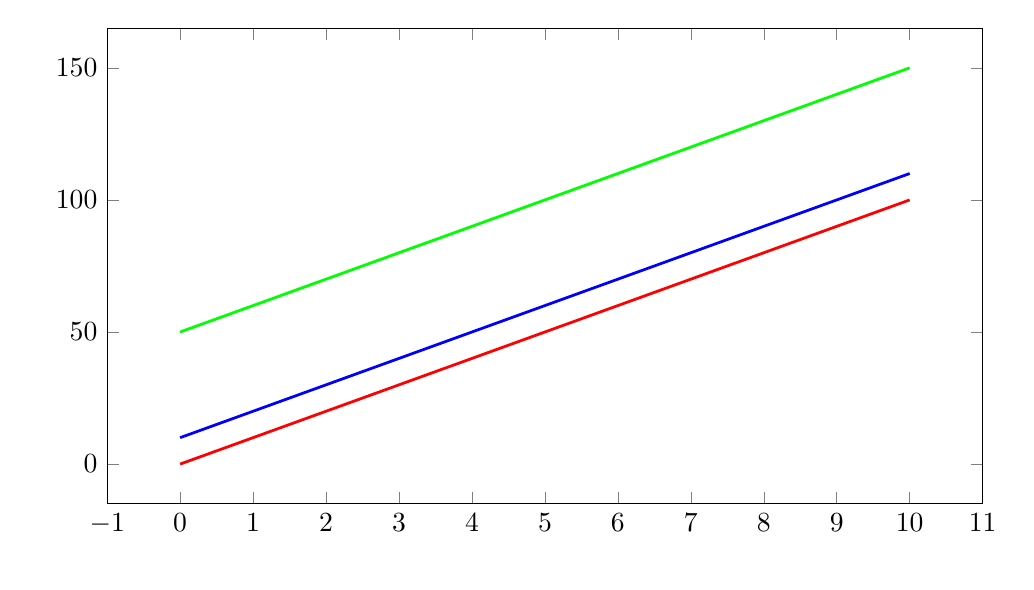
\begin{tikzpicture}[line width=1]
\begin{axis}[width=5in, height=3in,
             scatter/classes={a={mark=*,draw=black}},
             xlabel={\mbox{}},
             xlabel style={name=xlabel}, 
             ylabel={\mbox{}}, 
             legend style={
                at={(xlabel.south)},
                yshift=-1ex,
                anchor=north,
                legend cell align=left,
                },
        ]
]
\addplot[draw=red, line width=1] coordinates {(0.0,0.0)
(5.0,50.0)
(10.0,100.0)
(10.0,100.0)};\addplot[draw=blue, line width=1] coordinates {(0.0,10.0)
(5.0,60.0)
(10.0,110.0)
(10.0,110.0)};\addplot[draw=green, line width=1] coordinates {(0.0,50.0)
(5.0,100.0)
(10.0,150.0)
(10.0,150.0)};
\end{axis}\end{tikzpicture}\end{center}


(I'm not labeling the graphs
because you should be able to tell which is which ... right?)
For small values of $n$, i.e., $0 \leq n \leq 10$, the functions
are different and separated from each other.
But now if I increase the values for $n$, say, $0 \leq n \leq 100$, 
they look like this:
%-*-latex-*-

\begin{center}
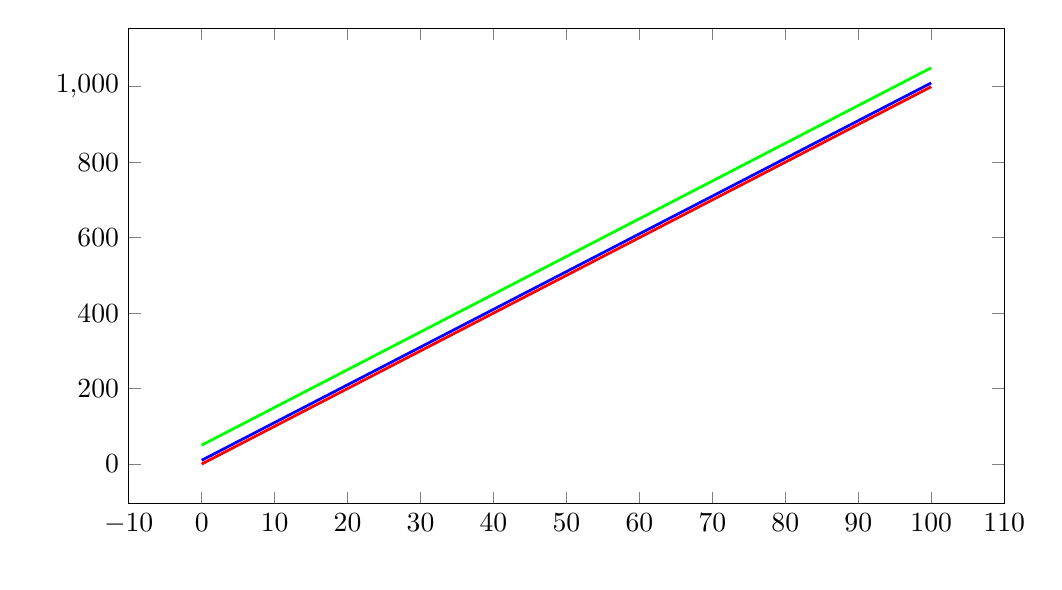
\begin{tikzpicture}[line width=1]
\begin{axis}[width=5in, height=3in,
             scatter/classes={a={mark=*,draw=black}},
             xlabel={\mbox{}},
             xlabel style={name=xlabel}, 
             ylabel={\mbox{}}, 
             legend style={
                at={(xlabel.south)},
                yshift=-1ex,
                anchor=north,
                legend cell align=left,
                },
        ]
]
\addplot[draw=red, line width=1] coordinates {(0.0,0.0)
(50.0,500.0)
(100.0,1000.0)
(100.0,1000.0)};\addplot[draw=blue, line width=1] coordinates {(0.0,10.0)
(50.0,510.0)
(100.0,1010.0)
(100.0,1010.0)};\addplot[draw=green, line width=1] coordinates {(0.0,50.0)
(50.0,550.0)
(100.0,1050.0)
(100.0,1050.0)};
\end{axis}\end{tikzpicture}\end{center}


And here's the plot for the domain of $0 \leq n \leq 1000$:
%-*-latex-*-

\begin{center}
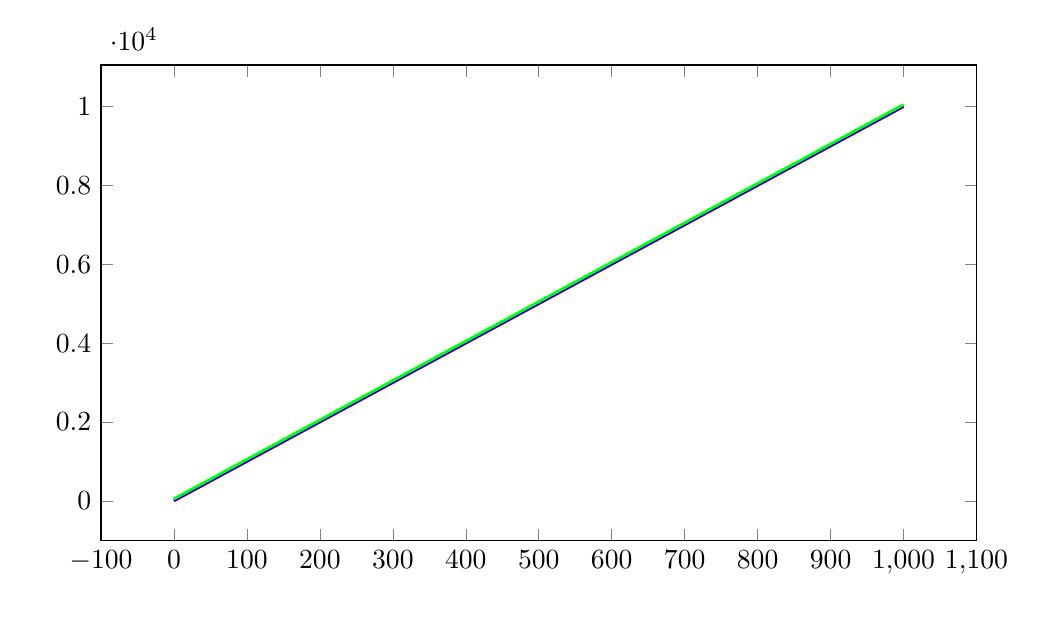
\begin{tikzpicture}[line width=1]
\begin{axis}[width=5in, height=3in,
             scatter/classes={a={mark=*,draw=black}},
             xlabel={\mbox{}},
             xlabel style={name=xlabel}, 
             ylabel={\mbox{}}, 
             legend style={
                at={(xlabel.south)},
                yshift=-1ex,
                anchor=north,
                legend cell align=left,
                },
        ]
]
\addplot[draw=red, line width=1] coordinates {(0.0,0.0)
(500.0,5000.0)
(1000.0,10000.0)
(1000.0,10000.0)};\addplot[draw=blue, line width=1] coordinates {(0.0,10.0)
(500.0,5010.0)
(1000.0,10010.0)
(1000.0,10010.0)};\addplot[draw=green, line width=1] coordinates {(0.0,50.0)
(500.0,5050.0)
(1000.0,10050.0)
(1000.0,10050.0)};
\end{axis}\end{tikzpicture}\end{center}

All three graphs more or less collapse into a single line, right?
You see that for large values of $n$,
the functions:
\[
y = 10n, \,\,\,\,\,
y = 10n + 10, \,\,\,\,\, 
y = 10n + 50
\]
really behave very much like each other: they all grow as fast as $10n$.

The second fudging step is when I throw away the $A$ 
in the function
\[
An
\]
and replace it by $1$ to get the function
\[
n
\]
because
the constant $A$ is hardware dependent
and has nothing to do with the inherent complexity of the
pseudocode.
If you change your machine, your $t_5$ will either larger or smaller.
On the other hand, the $n$ in $An$ is inherent to the pseudocode -- it comes
from the loop.
You cannot remove the loop (or the $n$) just by changing your machine.
%Here's a plot of $y = n$, $y = 10n$, $y = 100n$
%for $0 \leq n \leq 10$:
%%-*-latex-*-

\begin{center}
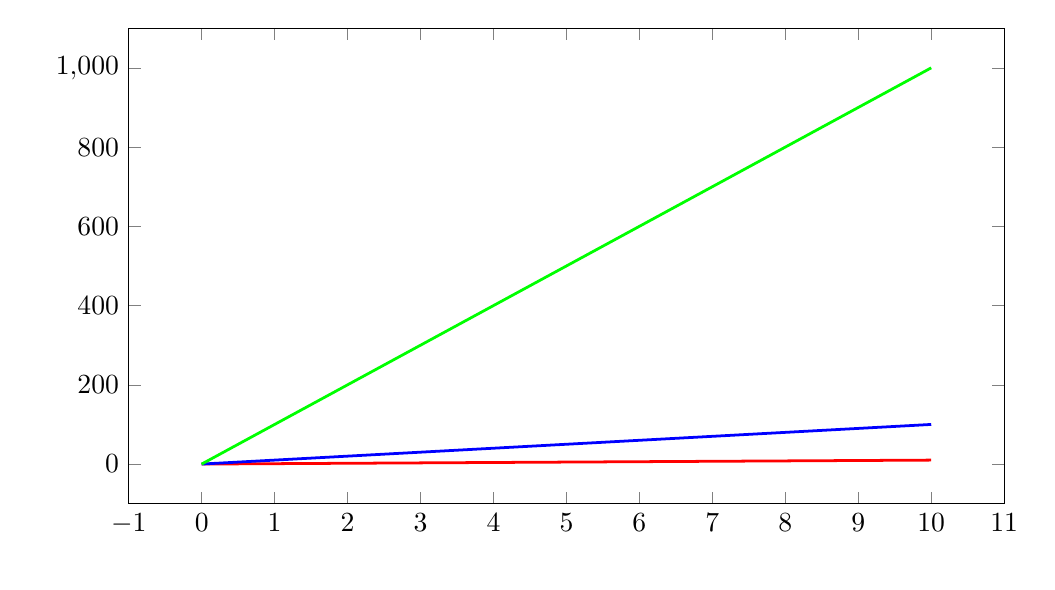
\begin{tikzpicture}[line width=1]
\begin{axis}[width=5in, height=3in,
             scatter/classes={a={mark=*,draw=black}},
             xlabel={\mbox{}},
             xlabel style={name=xlabel}, 
             ylabel={\mbox{}}, 
             legend style={
                at={(xlabel.south)},
                yshift=-1ex,
                anchor=north,
                legend cell align=left,
                },
        ]
]
\addplot[draw=red, line width=1] coordinates {(0.0,0.0)
(5.0,5.0)
(10.0,10.0)
(10.0,10.0)};\addplot[draw=blue, line width=1] coordinates {(0.0,0.0)
(5.0,50.0)
(10.0,100.0)
(10.0,100.0)};\addplot[draw=green, line width=1] coordinates {(0.0,0.0)
(5.0,500.0)
(10.0,1000.0)
(10.0,1000.0)};
\end{axis}\end{tikzpicture}\end{center}

%
%For $1000 \leq n \leq 10000$:
%%-*-latex-*-

\begin{center}
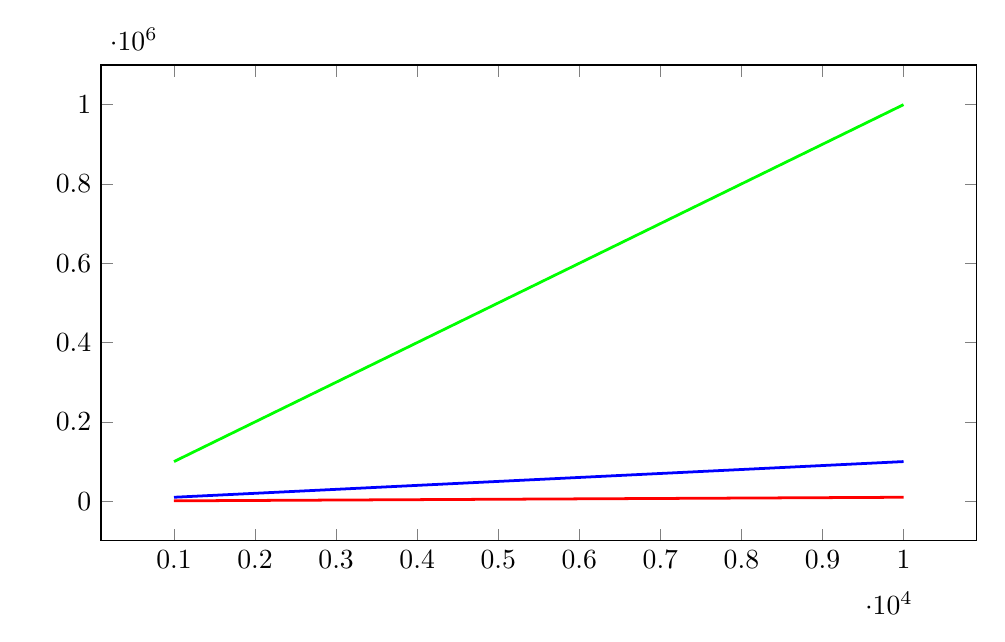
\begin{tikzpicture}[line width=1]
\begin{axis}[width=5in, height=3in,
             scatter/classes={a={mark=*,draw=black}},
             xlabel={\mbox{}},
             xlabel style={name=xlabel}, 
             ylabel={\mbox{}}, 
             legend style={
                at={(xlabel.south)},
                yshift=-1ex,
                anchor=north,
                legend cell align=left,
                },
        ]
]
\addplot[draw=red, line width=1] coordinates {(1000.0,1000.0)
(5500.0,5500.0)
(10000.0,10000.0)
(10000.0,10000.0)};\addplot[draw=blue, line width=1] coordinates {(1000.0,10000.0)
(5500.0,55000.0)
(10000.0,100000.0)
(10000.0,100000.0)};\addplot[draw=green, line width=1] coordinates {(1000.0,100000.0)
(5500.0,550000.0)
(10000.0,1000000.0)
(10000.0,1000000.0)};
\end{axis}\end{tikzpicture}\end{center}

%They are constant multiples of each other.
%And remember this important fact:
%I don't care about multiple differences since 
%in the case of functions measuring resource use (time in our case)
%it just mean that there's a difference in the hardware used.
Also,
you will see later that when we compare multiples of $n$ with
multiples of $n^2$ and multiples of $n^3$, you will see that the
when $n$ is huge,
multiples of $n$ clump together closely and away from the multiples of
$n^2$ and $n^3$.
You will also see that multiples of $n^2$ clump up together away from the 
multiples of $n^3$.
I'll show you some examples in the next section.

By the way, you can measure any resource taken up by an algorithm.
For instance you can also measure the \defone{space complexity} of an
algorithm, i.e., the amount of \textit{extra} memory needed to carry out 
an algorithm.

For the sum from 1 to $n$ algorithm, you are given $n$
and you need to store the result in $s$.
Any memory usage besides $n$ and $s$ (the memory
usage for input and output) is considered extra memory.
For our algorithm
\begin{Verbatim}[frame=single, fontsize=\footnotesize]
s = 0
for i = 1, 2, ..., n:
     s = s + i
\end{Verbatim}
The extra memory usage is due to variable $i$.
The variable \verb!s! is not considered extra -- you have to compute
\verb!s! since that's the goal of the algorithm.
Memory is frequently measured in bytes or bits.
(For serious theoretical CS, bits is used.)
Being an integer, $i$ might use up $4$ bytes.
I would then say the space complexity of our sum from 1 to $n$ algorithm is
\[
\textsc{Space}(n) = 4
\]
Since $4 = 4 \cdot n^0$, I will use the big-O notiation and write
\[
\textsc{Space}(n) = O(n^0) = O(1)
\]
In you prefer to use bits instead of bits, 4 bytes is 32 bits, which is then
\[
\textsc{Space}(n) = 32
\]
But $32 = 32 \cdot n^0$, so
\[
\textsc{Space}(n) = O(n^0) = O(1)
\]
which gives the same space complexity as when I use bytes to measure
memory usage.
It's also clear that you can also count the number of integer variables
(i.e., count 4-bytes) and arrive at the same space complexity.
In this case, I will say that the algorithm has
\defone{constant space complexity}.
Altogether for my sum from 1 to $n$ algorithm:
\begin{align*}
  T(n) &= O(n) \\
  \mathsc{Space}(n) &= O(1)
\end{align*}
  
%-*-latex-*-

\begin{ex} 
  \label{ex:prob-00}
  \tinysidebar{\debug{exercises/{disc-prob-28/question.tex}}}

  \solutionlink{sol:prob-00}
  \qed
\end{ex} 
\begin{python0}
from solutions import *
add(label="ex:prob-00",
    srcfilename='exercises/discrete-probability/prob-00/answer.tex') 
\end{python0}

%-*-latex-*-

\begin{ex} 
  \label{ex:prob-00}
  \tinysidebar{\debug{exercises/{disc-prob-28/question.tex}}}

  \solutionlink{sol:prob-00}
  \qed
\end{ex} 
\begin{python0}
from solutions import *
add(label="ex:prob-00",
    srcfilename='exercises/discrete-probability/prob-00/answer.tex') 
\end{python0}

%-*-latex-*-

\begin{ex} 
  \label{ex:prob-00}
  \tinysidebar{\debug{exercises/{disc-prob-28/question.tex}}}

  \solutionlink{sol:prob-00}
  \qed
\end{ex} 
\begin{python0}
from solutions import *
add(label="ex:prob-00",
    srcfilename='exercises/discrete-probability/prob-00/answer.tex') 
\end{python0}

%-*-latex-*-

\begin{ex} 
  \label{ex:prob-00}
  \tinysidebar{\debug{exercises/{disc-prob-28/question.tex}}}

  \solutionlink{sol:prob-00}
  \qed
\end{ex} 
\begin{python0}
from solutions import *
add(label="ex:prob-00",
    srcfilename='exercises/discrete-probability/prob-00/answer.tex') 
\end{python0}

%-*-latex-*-

\begin{ex} 
  \label{ex:prob-00}
  \tinysidebar{\debug{exercises/{disc-prob-28/question.tex}}}

  \solutionlink{sol:prob-00}
  \qed
\end{ex} 
\begin{python0}
from solutions import *
add(label="ex:prob-00",
    srcfilename='exercises/discrete-probability/prob-00/answer.tex') 
\end{python0}

%-*-latex-*-

\begin{ex} 
  \label{ex:prob-00}
  \tinysidebar{\debug{exercises/{disc-prob-28/question.tex}}}

  \solutionlink{sol:prob-00}
  \qed
\end{ex} 
\begin{python0}
from solutions import *
add(label="ex:prob-00",
    srcfilename='exercises/discrete-probability/prob-00/answer.tex') 
\end{python0}

